\input{../../preamble2.tex}

\begin{document}

\begin{titlepage}
    \vspace*{0pt}
    \vfill
    \centering
    \Huge\textbf{Интегралы и дифференциальные уравнения} \\[7pt]
    \Large\textbf{Лекции} \\
    \large 2 семестр \\ 
    \vfill
    \begin{flushright}
        \normalsize GitHub: \href{https://github.com/malyinik}{malyinik} \\
    \end{flushright}
    \normalsize 2024 г.
\end{titlepage}
\newpage

\tableofcontents
\newpage

%%%%%%%%

\section{Первообразная и неопределённый интеграл}

\subsection{Первообразная}
\begin{definition}\hlabel{опр: первообразная}
    Функция $F(x)$ называется \textbf{первообразной} функции $f(x)$ на интервале $(a;b)$, если $F(x)$ дифференцируема на $(a;b)$ и $\forall x \in (a;b)\colon$
    \begin{gather}
        \boxed{F'(x) = f(x)}
    \end{gather}
\end{definition}
\begin{eg}
    \begin{flalign*}
        & f(x) = \frac{1}{2\sqrt{x}},\ D_f = (0; +\infty) &\\
        & F(x) = \sqrt{x} \text{ --- первообразная } f(x) = \frac{1}{2\sqrt{x}} &\\
        & F'(x) = (\sqrt{x})' = \frac{1}{2\sqrt{x}} = f(x) &\\
        & F(x) = \sqrt{x} + 3 \text{ --- первообразная } f(x) = \frac{1}{2\sqrt{x}} &
    \end{flalign*}
\end{eg}

\subsubsection{Свойства первообразной}

    \begin{property}
        Если $F(x)$ --- первообразная функции $f(x)$ на $(a;b)$, то $F(x) + C$ --- первообразная функции $f(x)$ на $(a;b)$, где $\forall C$ --- $const$.
    \end{property}
    \begin{property}
        \sloppy Если $\varPhi(x)$ дифференцируема на $(a;b)$ и $\forall x \in (a;b)\colon \varPhi'(x) = 0$, то $\varPhi (x) = const$, ${\forall x \in (a;b)}$.
    \end{property}
    \begin{property}[Существование первообразной]
        Любая непрерывная функция на $(a;b)$ имеет множество первообразных на этом интервале, причём любые две из них отличаются друг от друга на константу.
        \begin{gather*}
            \varPhi(x),\ F(x) \text{ --- первообразные функции } f(x) \text{ на } (a;b) \\
            \varPhi(x) - F(x) = const
        \end{gather*}
    \end{property}

\newpage
\subsection{Неопределённый интеграл}

\begin{definition}\hlabel{опр: неопределённый интеграл}
    Множество первообразных функции $f(x)$ на $(a;b)$ называется \textbf{неопределённым интегралом}.
    \begin{gather}
        \boxed{\int f(x)dx = F(x) + C}
    \end{gather}
    $\int$ --- знак интеграла\\
    $f(x)$ --- подынтегральная функция\\
    $f(x)dx$ --- подынтегральное выражение\\
    $x$ --- переменная\\
    $F(x) + C$ --- множество первообразных\\
    $C$ --- произвольная константа
\end{definition}

\begin{definition}
    \textbf{Интегрирование} --- нахождение неопределённого интеграла.
\end{definition}

\subsubsection{Свойства неопределённого интеграла}
\setcounter{property}{0}

\begin{property}
    Производная от неопределённого интеграла равна подынтегральной функции.
    \begin{gather*}
        \boxed{\left(\int{f(x)dx}\right)' = f(x)}
    \end{gather*}
\end{property}
\begin{proof}
    \begin{gather*}
        \left(\int f(x)dx\right)' \xlongequal{(\ref{опр: неопределённый интеграл})} \big(F(x) + C\big)' = F'(x) + C' = F'(x) \xlongequal{(\ref{опр: первообразная})} f(x)
    \end{gather*}
\end{proof}

\begin{property}
    Дифференциал от неопределённого интеграла равен подынтегральному выражению.
    \begin{gather*}
        \boxed{d\left(\int f(x)dx\right) =  f(x)dx}
    \end{gather*}
\end{property}
\begin{proof}[Докво]
    \begin{gather*}
        d\left(\int f(x)dx\right) \xlongequal{(\ref{опр: неопределённый интеграл})} d\big(F(x) + C\big) = \big(F(x) + C\big)'dx = \big(F'(x) + C'\big)dx = F'(x)dx \xlongequal{(\ref{опр: первообразная})} f(x)dx
    \end{gather*}
\end{proof}

\newpage
\begin{property}\hlabel{св: неопределённый интеграл 3}
    Неопределённый интеграл от дифференциала от некоторой функции равен сумме этой функции и константы.
    \begin{gather*}
        \boxed{\int d\big(F(x)\big) = F(x) + C},\quad \forall C \text{ --- } const
    \end{gather*}
\end{property}
\begin{proof}
    \begin{gather*}
        \int d\big(F(x)\big) = \int F'(x)dx \xlongequal{(\ref{опр: первообразная})} \int f(x)dx \xlongequal{\text{(\ref{опр: неопределённый интеграл})}} F(x) + C,\quad \forall C \text{ --- } const
    \end{gather*}
\end{proof}

\begin{property}
    Константу можно выносить за знак неопределённого интеграла.
    \begin{gather*}
        \boxed{\int \lambda\cdot f(x)dx = \lambda \int f(x)dx},\quad \lambda \ne 0
    \end{gather*}
\end{property}
\begin{proof}
    Пусть $F(x)$ --- первообразная $f(x)$
    \begin{gather*}
        \lambda \int f(x)dx \xlongequal{(\ref{опр: неопределённый интеграл})} \lambda \cdot \big(F(x) + C\big),\quad \forall C \text{ --- } const
    \end{gather*}
    Функция $\lambda \cdot F(x)$ --- первообразная $\lambda \cdot f(x)\colon$
    \begin{gather*}
        \big(\lambda \cdot F(x)\big)' = \lambda\cdot F'(x) \xlongequal{(\ref{опр: первообразная})} \lambda\cdot f(x)\\
        \int \lambda\cdot f(x)dx \xlongequal{(\ref{опр: неопределённый интеграл})} \lambda\cdot F(x) + C_1,\quad \forall C_1 \text{ --- } const
    \end{gather*}
    Так как константы $C_1,\ C$ --- произвольные, $\lambda \ne 0$, то их всегда можно выбрать так, чтобы $C_1 = \lambda C$. Тогда множества $\lambda\cdot\big(F(x) + C\big)$ и $\lambda\cdot F(x) + C_1$ совпадают.
\end{proof}

\begin{property}
    Если функции $f_1(x)$ и $f_2(x)$ на $(a;b)$ имеют первообразные $F_1(x)$ и $F_2(x)$ соответственно, то функция $\lambda_1 f_1(x) + \lambda_2 f_2(x)$, где $\lambda_1, \lambda_2 \in \R$, имеет первообразную на $(a;b)$, причём $\lambda_1^2 + \lambda_2^2 > 0\colon$
    \begin{gather*}
        \int\Big(\lambda_1 f_1(x) + \lambda_2 f_2(x)\Big)dx = \lambda_1 \int f_1(x)dx + \lambda_2 \int f_2(x)dx
    \end{gather*}
\end{property}
\begin{proof}
    $F_1(x)$ --- первообразная $f_1(x)$\\
    $F_2(x)$ --- первообразная $f_2(x)$\\
    \begin{align*}
        \lambda_1 \int f_1(x)dx + \lambda_2 \int f_2(x)dx &\xlongequal{(\ref{опр: неопределённый интеграл})} \lambda_1 (F_1(x) + C_1) + \lambda_2 \big(F_2(x) + C_2\big) = \\
        &= \lambda_1 F_1(x) + \lambda_2 F_2(x) + \lambda_1 C_1 + \lambda_2 C_2,\quad \forall C_1, C_2 \text{ --- } const
    \end{align*}
    Функция $F(x) = \lambda_1 F_1(x) + \lambda_2 F_2(x)$ --- первообразная функции $\lambda_1 f_1(x) + \lambda_2 f_2 (x)$.
    \begin{gather*}
        F'(x) = \big(\lambda_1 F_1(x) + \lambda_2 F_2 (x)\big)' = \lambda_1 F_1'(x) + \lambda_2 F_2'(x) \xlongequal{(\ref{опр: первообразная})} \lambda_1 f_1(x) + \lambda_2 f_2(x)\\
        \int \Big(\lambda_1 f_1(x) + \lambda_2 f_2(x)\Big)dx \xlongequal{(\ref{опр: неопределённый интеграл})} \lambda_1 f_1(x) + \lambda_2 f_2(x) + C,\quad \forall C \text{ --- } const
    \end{gather*}
    Так как константы $C_1,\ C_2,\ C$ --- произвольные, то всегда можно добиться выполнения равенства $C = \lambda_1 C_1 + \lambda_2 C_2$. \\
    Тогда множества $\lambda_1 F_1(x) + \lambda_2 F_2(x) + \lambda_1 C_1 + \lambda_2 C_2$ и $\lambda_1 F_1(x) + \lambda_2 F_2(x) + C$ совпадают.
\end{proof}

\begin{property}[Инвариантность формы интегрирования]
    Если $\int f(x)dx = F(x) + C$, где $C$ --- $const$, то $\int f(u)du = F(u) + C$, где $C$ --- $const$, ${u = \varphi (x)}$ --- непрерывно-дифференцируемая функция.
\end{property}
\begin{proof}
    $x$ --- независимая переменная\\
    $f(x)$ --- непрерывная функция\\
    $F(x)$ --- первообразная $f(x)$\\[1ex]
    $\displaystyle \int f(x)dx = F(x) + C,\ \forall C$ --- $const$\\[1ex]
    Рассмотрим сложную функцию $F(u) = F\big(\varphi(x)\big)$. Найдём дифференциал $F(u)$:
    \begin{gather*}
        d\big(F(u)\big) = F'(u)\cdot \underbrace{\varphi'(x)dx}_{du} = \left|\begin{aligned} u &= \varphi (x)\\ du &= \varphi'(x)dx \end{aligned}\right| = F'(u)du \xlongequal{(\ref{опр: первообразная})} f(u)du
    \end{gather*}
    Неопределённый интеграл:
    \begin{gather*}
        \int f(u)du = \int d\big(F(u)\big) \xlongequal{\textbf{(св. \ref{св: неопределённый интеграл 3})}} F(u) + C,\quad \forall C \text{ --- } const
    \end{gather*}
\end{proof}

\begin{eg}
    \begin{flalign*}
        & \int \sin x dx = -\cos x + C\qquad \sin (2x) d(2x) = -\cos(2x) + C &
    \end{flalign*}
\end{eg}

\subsubsection{Геометрический смысл}
Неопределённый интеграл геометрически представляет собой семейство интегральных кривых (графиков функций) вида $y = F(x) + C,\ \forall C$ --- $const$.
\begin{figure}[h]
    \centering
    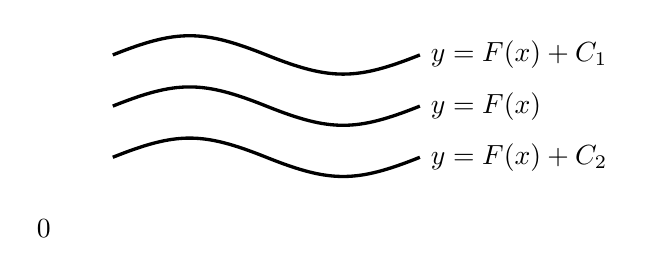
\begin{tikzpicture}[very thick, scale=0.65]
        \tkzInit[xmin=-1, xmax=7, ymin=-1, ymax=3]
        \tkzDrawX[thick] \tkzDrawY[thick]
        \node[below left] at (0, 0) {$0$};
        
        \draw (1, 1) .. controls (2.25, 1.5) and (2.75, 1.5) .. (4, 1) .. controls (5.25, 0.5) and (5.75, 0.5).. (7, 1) node[right]{$y=F(x) + C_2$};
        \draw (1, 2) .. controls (2.25, 2.5) and (2.75, 2.5) .. (4, 2) .. controls (5.25, 1.5) and (5.75, 1.5).. (7, 2) node[right]{$y=F(x)$};
        \draw (1, 3) .. controls (2.25, 3.5) and (2.75, 3.5) .. (4, 3) .. controls (5.25, 2.5) and (5.75, 2.5).. (7, 3) node[right]{$y=F(x) + C_1$};
    \end{tikzpicture}
    \caption{Геометрический смысл неопределённого интеграла}
\end{figure}
    
\subsubsection{Таблица основных интегралов}

\begin{table}[h]
    \caption{Таблица основных интегралов}
    \centering
    \begin{tabular}{|ll|}
        \hline
         & \\[-8pt]
        1. $\displaystyle \int x^n dx = \frac{x^{n+1}}{n+1} + C,\ \forall C \text{ --- } const$ & 11. $\displaystyle \int \frac{dx}{a^2 - x^2} = \frac{1}{2a}\ln \left| \frac{a+x}{a-x} \right| + C$ \\[2ex]
        2. $\displaystyle \int dx = x + C$ & 12. $\displaystyle \int \frac{dx}{x^2 - a^2} = \frac{1}{2a}\ln \left| \frac{a-x}{a+x} \right| + C$ \\[2ex]
        3. $\displaystyle \int \frac{dx}{x} = \ln |x| + C$ & 13. $\displaystyle \int \frac{dx}{\sqrt{a^2 - x^2}} = \arcsin \frac{x}{a} + C$ \\[2ex]
        4. $\displaystyle \int e^x dx = e^x + C$ & 14. $\displaystyle \int \frac{dx}{\sqrt{x^2 \pm a^2}} = \ln \left|x + \sqrt{x^2 \pm a^2}\right| + C$ \\[2ex]
        5. $\displaystyle \int a^xdx = \frac{a^x}{\ln a} + C$ & 15. $\displaystyle \int \sh x\ dx = \ch x + C$\\[2ex]
        6. $\displaystyle \int \sin x\ dx = -\cos x + C$ & 16. $\displaystyle \int \ch x\ dx = \sh x + C$ \\[2ex]
        7. $\displaystyle \int \cos x\ dx = \sin x + C$ & 17. $\displaystyle \int \frac{dx}{\ch^2x} = \th x + C$ \\[2ex]
        8. $\displaystyle \int \frac{dx}{\cos^2x} = \tg x + C$ & 18. $\displaystyle \int \frac{dx}{\sh^2x} = - \cth x + C$\\[2ex]
        9. $\displaystyle \int \frac{dx}{\sin^2x} = -\ctg x + C$ & 19. $\displaystyle \int \frac{dx}{\sin x} = \ln \left| \tg \frac{x}{2} \right| + C$ \\[2ex]
        10. $\displaystyle \int \frac{dx}{a^2 + x^2} = \frac{1}{a}\arcctg \frac{x}{a} + C$ & 20. $\displaystyle \int \frac{dx}{\cos x} = \ln \left| \tg \left(\frac{x}{2} + \frac{\pi}{4}\right) \right| + C$ \\[2ex]
        \hline
    \end{tabular}
\end{table}
\vspace{20pt}
\begin{proof}[][19]
    \begin{flalign*}
        \int \frac{dx}{\sin x} &= \int \frac{dx}{2 \sin \dfrac{x}{2} \cos \dfrac{x}{2}} = \frac{1}{2}  \int \frac{\dfrac{1}{\cos^2 \frac{x}{2}}}{\dfrac{\sin \frac{x}{2} \cancel{\cos \frac{x}{2}}}{\cos^{\cancel{2}} \frac{x}{2}}}dx = \int \frac{\dfrac{1}{2\cos^2 \frac{x}{2}}}{\tg \frac{x}{2}}dx = \int \frac{d\left(\tg \frac{x}{2}\right)}{\tg \frac{x}{2}} = &\\
        &= \left| \tg \frac{x}{2} t \right| = \int \frac{dt}{t} = \ln |t| + C = \ln \left| \tg \frac{x}{2} \right| + C &
    \end{flalign*}
\end{proof}

\newpage
\subsection{Основные методы интегрирования}
\begin{enumerate}
    \item Непосредственное интегрирование (свойства + таблица)
    \begin{eg}
        \begin{flalign*}
            \int\left(3e^x + \sin x - \frac{1}{1 + x^2}\right)dx &= 3\int e^xdx + \int \sin x\ dx - \int \frac{dx}{1+x^2} = &\\
            &= 3e^x - \cos x - \arctg x + C,\ \forall C \text{ --- } const &
        \end{flalign*}
    \end{eg}
    \item Метод подстановки
    \begin{enumerate}
        \item Занесение под знак дифференциала
        \begin{eg}
            \begin{flalign*}
                & \int \frac{e^{\arcsin x} \cdot 1}{\sqrt{1 - x^2}}dx = \int e^{\arcsin x} d (\arcsin x) = e^{\arcsin x} + C,\ \forall C \text{ --- } const
            \end{flalign*}
        \end{eg}
        \item Замена переменной\\
        Пусть функция $x = \varphi (t)$ определена и дифференцируема на $T$, а множество $X$ --- множество значений этой функции, на котором определена $f(x)$. Тогда, если существует первообразная функции $f(x)$ на $X$, то на множестве $T$ верно равенство:
        \begin{gather*}
            \boxed{\int f(x) dx = \left|\begin{aligned} x &= \varphi (t) \\ dx &= \varphi'(t) \end{aligned}\right| = \int f\big(\varphi(t)\big)\varphi'(t)dt}
        \end{gather*}
        \begin{eg}
            \begin{flalign*}
                & \int x(3x - 1)^{2024}dx = \left| \begin{aligned} & 3x - 1 = t\quad 3x = t + 1 \\ & x = \frac{1}{3}\big(t + 1\big) \\ & dx = \left(\frac{1}{3}t + \frac{1}{3}\right)'dt = \frac{1}{3}dt \end{aligned} \right| = \int \frac{1}{3}\big(t + 1\big) \cdot t^{2024}\frac{1}{3}dt&
            \end{flalign*}
        \end{eg}
    \end{enumerate} 
\end{enumerate}



%%%%%%
\end{document}